\chapter{Experiment Description }

Modern general-purpose detectors used in high-energy colliders typically employ cylindrical detection layers arranged around the beam axis. One such example is the Compact Muon Solenoid (CMS), which is part of the Large Hadron Collider (LHC) at CERN and is considered one of the largest international scientific collaborations in history. The CMS detector is 15 meters tall and 21 meters long, and is designed for a broad physics program that includes studying the Standard Model. This chapter provides a description of the various components of the CMS detector, with a particular focus on the silicon pixel tracker, which is described in greater detail due to its relevance to the thesis.
 

\section{The Compact Muon Solenoid}

The Compact Muon Solenoid (CMS) experiment is one of the four general-purpose detectors situated at the Large Hadron Collider (LHC). The CMS detector is constructed around a massive solenoid magnet, which is a cylindrical coil of superconducting cable generating a field of 4 tesla, this field is used to separate the calorimeter energy deposits of charged and neutral particles in jets. The field is confined by a steel "yoke" which constitutes the bulk of the detector's weight of 14,000 tonnes. 

The CMS detector has a complete length of 21.6 meters and a diameter of 14.6 meters that  comprises various detection layers that include separate parts of the detector. These layers are the fine-grained silicon tracker, which provides efficient and precise reconstruction of charged-particle trajectory. The highly-segmented electromagnetic calorimeter (ECAL) can separate energy deposits from particles in jets with high resolution. The hadronic calorimeter (HCAL) has a coarse segmentation, but it is still sufficient to distinguish between charged and neutral hadron energy deposits in jets. Additionally, there is an excellent muon tracking system, which delivers efficient and pure muon identification regardless of the surrounding particles. A schematic representation of the CMS detector is shown in \ref{detector_CMS}.\.

\begin{center}
  \begin{figure}[ht]
    \centering
    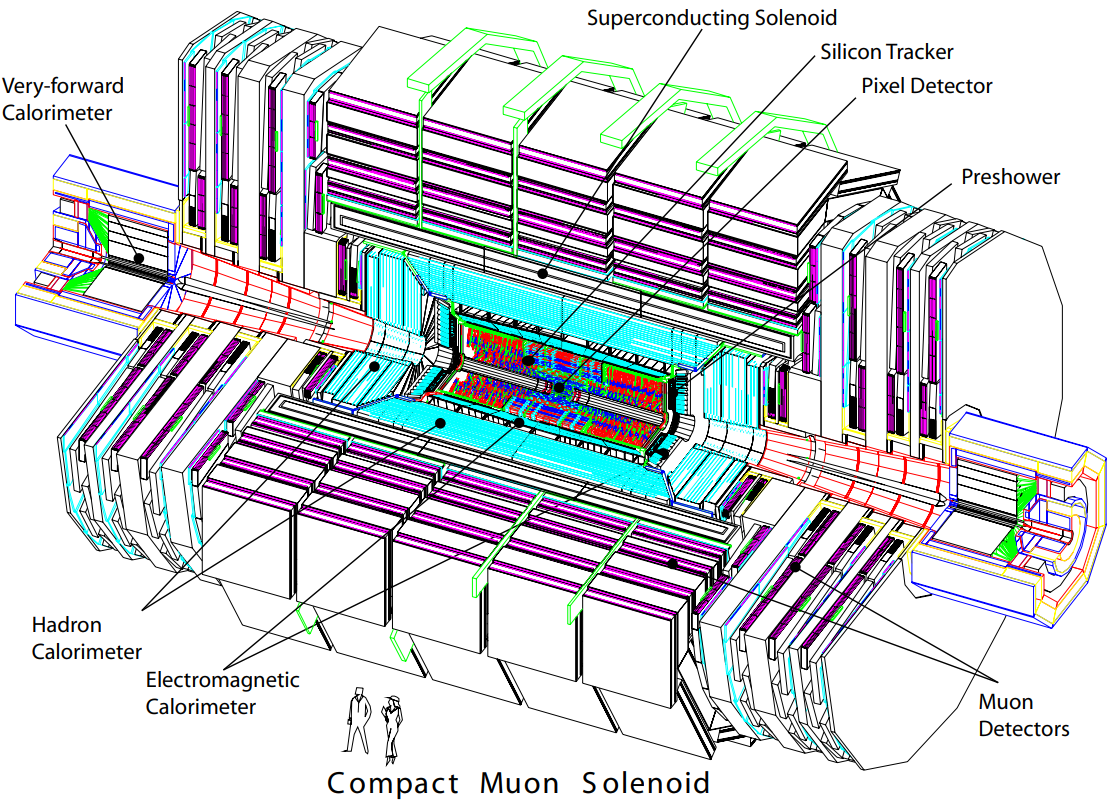
\includegraphics[scale=.3]{Chapter2/CMS_detector_simple.png}
    \caption[Perspective view of the CMS detector]{Perspective view of the CMS detector.}
    \label{detector_CMS}
  \end{figure}
\end{center}

A powerful magnet is required to bend charged particles as they travel outward from the collision point. Bending the trajectory of the particles serves two purposes: first, it helps identify the charge of the particle, as positively and negatively charged particles bend in opposite directions in the same magnetic field; and second, it enables measurement of the particle's momentum.

The CMS must identify the paths of these deflected charged particles with high precision. This is achieved using a silicon tracker composed of approximately 75 million individual electronic sensors arranged in concentric layers. When a charged particle passes through a Tracker layer, it interacts electromagnetically with the silicon and produces a hit. These individual hits can be combined to identify the track of the traversing particle.

The energies of the particles are crucial to understanding what occurred at the collision point. This information is collected from two calorimeters in the CMS. The inner layer is the Electromagnetic Calorimeter (ECAL), which measures the energy of electrons and photons by completely stopping them. It is a hermetic, homogeneous calorimeter consisting of 61,200 lead tungstate (PbWO4) crystals mounted in the central barrel part and closed by 7,324 crystals in each of the two endcaps. In front of the endcap crystals, a preshower detector is placed. Avalanche photodiodes (APDs) are used as photodetectors in the barrel and vacuum phototriodes (VPTs) in the endcaps. Hadrons, which are composite particles made up of quarks and gluons, travel through the ECAL and are stopped by the outer layer, called the Hadron Calorimeter (HCAL).

The final particle that the CMS directly observes is the muon. Muons are approximately 200 times heavier than electrons and are not stopped by the calorimeters. Therefore, special sub-detectors have to be constructed to detect them as they traverse the CMS. These sub-detectors are interleaved with the return yoke of the solenoid. The large magnet of the CMS also allows us to measure each muon's momentum both inside the superconducting coil (using the tracking devices) and outside of it (using the muon chambers). A transverse slice of the CMS detector, depicting specific particle interactions, is shown in Figure \ref{slice_CMS}.


\begin{center}
  \begin{figure}[ht]
    \centering
    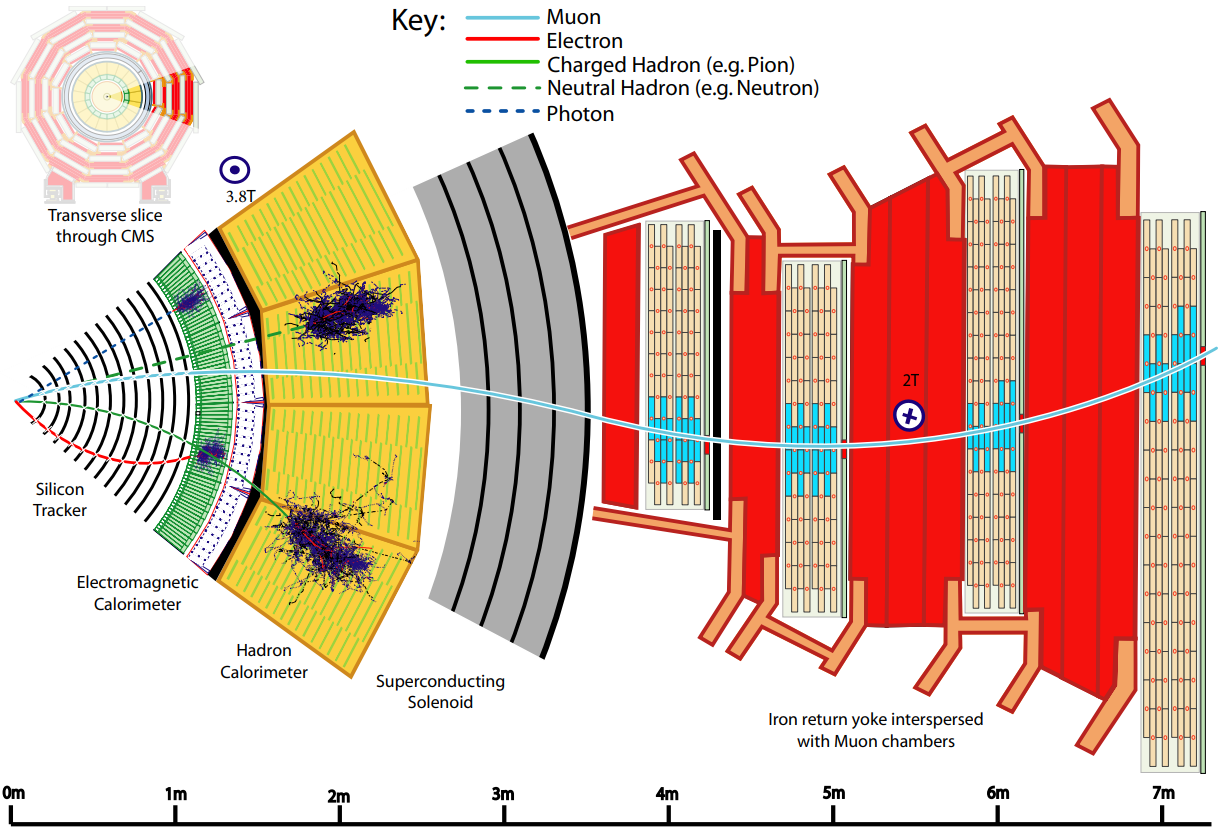
\includegraphics[scale=.3]{Chapter2/slice_det.png}
    \caption[Transverse slice fo CMS detector]{Sketch of a transverse slice of the CMS detector with specific particle interactions, from the beam interaction region to the muon detector. The muon and the charged pion are positively charged, and the electron is negatively charged \cite{det_summary}.}
    \label{slice_CMS}
  \end{figure}
\end{center}

The coordinate system adopted by CMS has the origin at the center of the detector, the $y$-axis pointing vertically upward, and the $x$-axis pointing radially inward toward the center of the LHC. Thus, the z-axis points along the beam direction toward the Jura mountains from LHC Point 5. The azimuthal angle $\varphi$ is measured from the $x$-axis in the $x-y$ plane and the radial coordinate in this plane is denoted by $r$. The polar angle $\theta$ is measured from the $z$-axis. Pseudorapidity is defined as $\eta=- \ln \tan (\theta/2)$ \cite{CMS_Exp_2008}.\\

\section{CMS Tracking System}

The tracking system plays a crucial role in precisely measuring the trajectories and momenta of charged particles generated by collisions in the LHC, as well as reconstructing secondary vertices. It has a physical size of 5.8 m in length and 2.5 m in diameter and is surrounded by the CMS solenoid, which provides a homogeneous magnetic field of 4 T throughout the tracker's volume.

The CMS tracker consists of two parts: a pixel detector with three barrel layers located between 4.4 cm and 10.2 cm radii and a silicon strip tracker with ten barrel detection layers extending to a radius of 1.1 m. Each part includes endcaps, with the pixel detector having two disks and the strip tracker having three plus nine disks on each side of the barrel. This extends the tracker's acceptance up to a pseudorapidity of $|\eta| < 2.5$, with an active silicon area of approximately 200 $m^2$. The construction of the CMS tracker required the development of new production methods and quality control procedures in order to produce its 1440 pixel and 15148 strip detector modules. The layout of the CMS tracker is presented in the following figure:

\begin{center}
  \begin{figure}[ht]
    \centering
    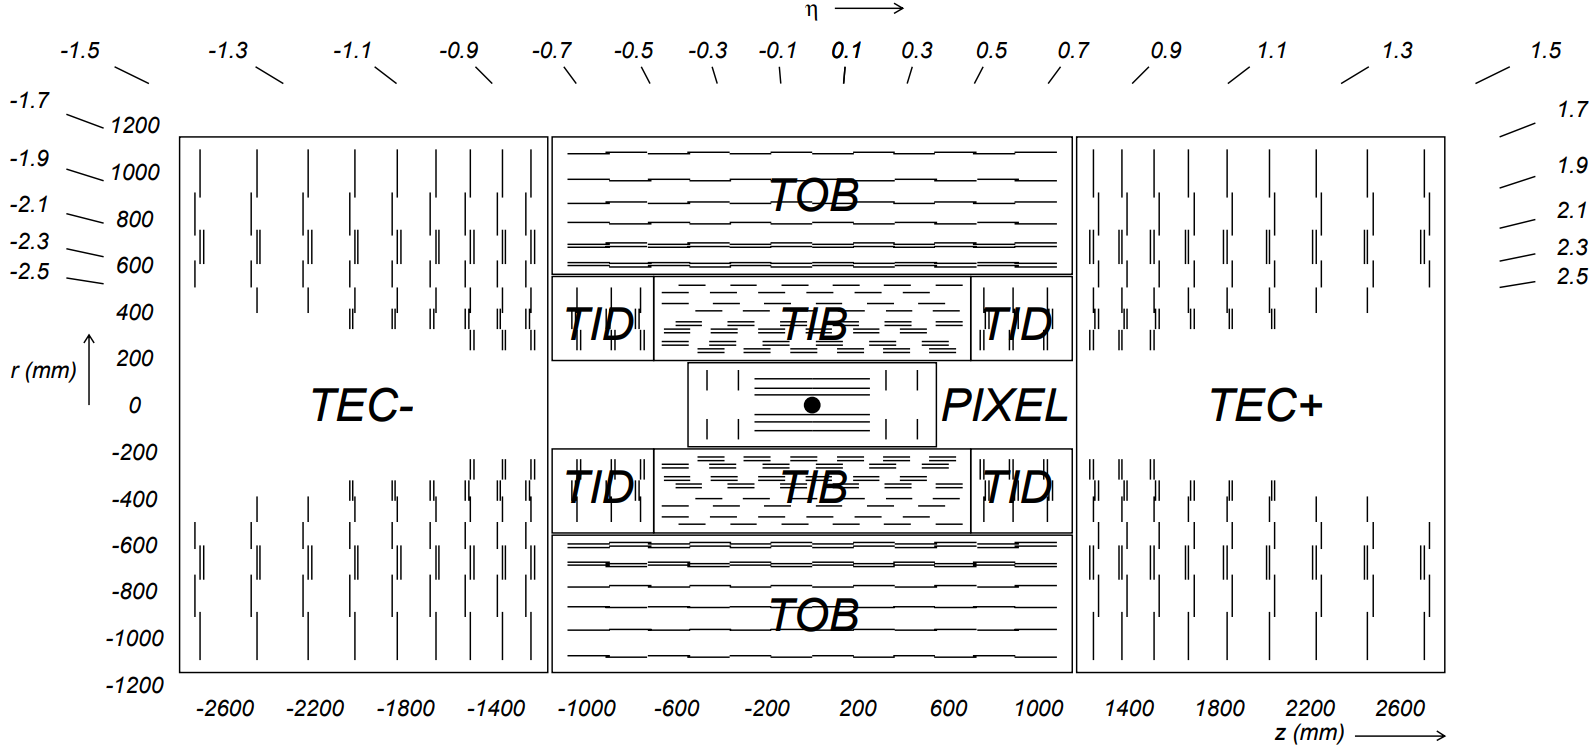
\includegraphics[scale=.23]{Chapter2/strip_layout.png}
    \caption[Schematic cross section through the CMS tracker]{Schematic cross section through the CMS tracker. Each line represents a detector module \cite{CMS_Exp_2008}. The Pixel tracker here is not the CMS Phase-1 pixel detector.}
    \label{strip_layout}
  \end{figure}
\end{center}

As a charged particle traverses a medium, it creates a trail of ionized atoms and liberated electrons. By detecting this ionization, it is possible to reconstruct the trajectory of the charged particle. In each cylindrical layer of a silicon sensor, a charged particle will leave a hit, which enables the reconstruction of the charged particle track \cite{thomson_2013}.

The interaction of a charged particle with a medium results in electromagnetic interaction with the atomic electrons, leading to energy loss through atomic ionization \cite{thomson_2013}. The theory governing such losses is predominantly due to Coulomb scattering from the atomic electrons, which was established by Bethe, Bloch, and others in the 1930s. The resulting formula, known as the Bethe-Bloch formula, is expressed as \cite{Martin2017_book}:

\begin{equation}
  -\frac{dE}{dx}= \frac{Dq^{2}n_{e}}{\beta ^{2}} \biggl[ \ln \left(\frac{2m_{e}c^{2}\gamma^{2}}{I} \right) -\beta^{2} -\frac{\delta(\gamma)}{2}  \biggr]
  \label{bethe}
\end{equation}

$x$ is the distance travelled through the medium, $m_{e}$ is the electron mass, $\beta=v/c$,  $\gamma =(1-\beta^{2})^{-1/2}$ and $D=\frac{4\pi \alpha^{2} \hslash^{2}}{m_{e}}=$5.1$\times 10^{-25}$MeV cm$^{2}$. The other constants refers to the medium: $n_{e}$ is the electron density, $I$ is the mean ionisation potencial of the atoms averaged over all electrons (given approximately by $I$=10$Z$eV for $Z>$20) and $\delta$ is a dielectric screening correction that is only important for highly relativistic particles. 

The CMS tracking detector relies on semiconductor technology that uses silicon pixels and strips. This tracking system is made up of two subsystems: the pixel tracker, which is the closest to the interaction point, and the strip tracker \cite{CMS_Exp_2008}. The following section will provide a description of the pixel detector.

\subsection{Pixel Detector and Clustering}
\label{pixel_clust_reco}

The CMS experiment conducted at the Large Hadron Collider (LHC) at CERN comprises a silicon pixel detector, which forms the innermost component of the tracking system. This detector facilitates the provision of 3-dimensional space points in the area nearest to the interaction point, which, in turn, enables precise tracking of charged particles and vertex reconstruction. The pixel detector operates in a radiation-rich environment, marked by high track density.

The CMS pixel detector encompasses four concentric barrel layers (L1-L4), each with radii measuring 29, 68, 109, and 160 mm, and three disks (D1-D3) on either end positioned at distances of 291, 396, and 516 mm from the detector's center. A schematic of the CMS Phase-1 pixel detector's arrangement is depicted in Figure \ref{phase1_pixel_detector} where the total silicon area of the CMS Phase-1 pixel detector spans 1.9 square meters. The pixel detector comprises 1856 segmented silicon sensor modules, with 1184 modules used in the barrel pixel detector (BPIX) and 672 modules in the forward disks (FPIX). Each module features a sensor with 160 by 416 pixels, connected to 16 readout chips (ROCs), resulting in 124 million readout channels in total.

\begin{center}
  \begin{figure}[h]
    \centering
    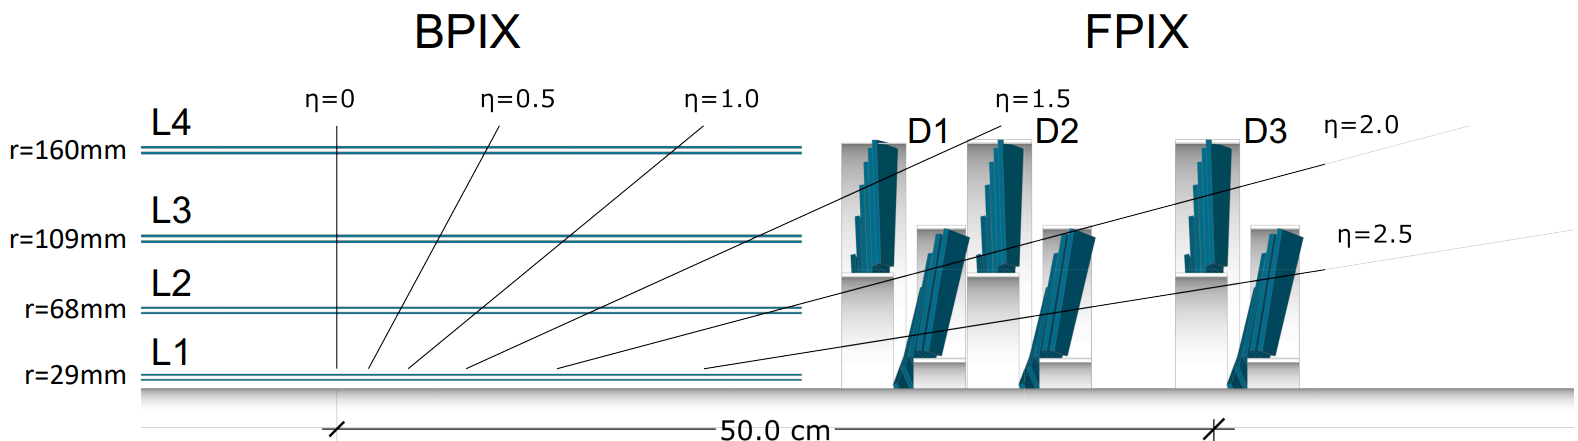
\includegraphics[scale=.26]{Chapter2/phase1_PixelDetector.png}
    \caption[CMS Phase-1 pixel detector]{Layout of the CMS Phase-1 pixel detector in longitudinal view\cite{phase1_Pixel_Detector}.}
    \label{phase1_pixel_detector}
  \end{figure}
\end{center}

The BPIX and FPIX detectors are equipped with four service half-cylinders each, with a combined length of 540 mm. These cylinders host the readout and control circuits, and provide guidance for the power lines and cooling tubes of the detector. The BPIX detector is bifurcated into two mechanically self-sufficient halves, both of which are made up of a half detector and two service half-cylinders. The orientation of the sensor surface of the modules in both halves is parallel to the magnetic field.
On the other hand, the FPIX detector is segmented into four mechanically independent quadrants, each of which comprises three half-disks housed in a service half-cylinder. The sensor orientation in the FPIX detector is arranged such that the long side of the pixel is aligned with the radial direction and has a coverage from 45 to 161 mm. The half-disks are additionally subdivided into inner and outer half-rings that support 22 and 34 modules, respectively.\\

The CMS Phase-1 pixel detector is built from 1856 segmented silicon sensor modules, where 1184 modules are used in the barrel pixel detector (BPIX) and 672 modules are used for the forward disks (FPIX). Each module consists of a sensor with 160$\times$416 pixels connected to 16 readout chips (ROCs). In total there are 124 million readout channels \cite{phase1_Pixel_Detector}.
A pixel detector module is built from a planar silicon sensor with a size of 18.6 $\times$ 66.6 $\text{mm}^{2}$ (active area of 16.2 $\times$ 64.8 $\text{mm}^{2}$), bump-bonded to an array of 2$\times$8 ROCs. Each ROC is segmented into 4160 readout channels and reads out the pulse height information for each pixel. The standard pixel size is 100$\times$150 $\mu m^{2}$, as in the original pixel detector.
The figures depicting the modules of the CMS Phase-1 pixel detector can be found in Figure \ref{modules_drawing} \cite{phase1_Pixel_Detector}.

\begin{center}
  \begin{figure}[h]
    \centering
    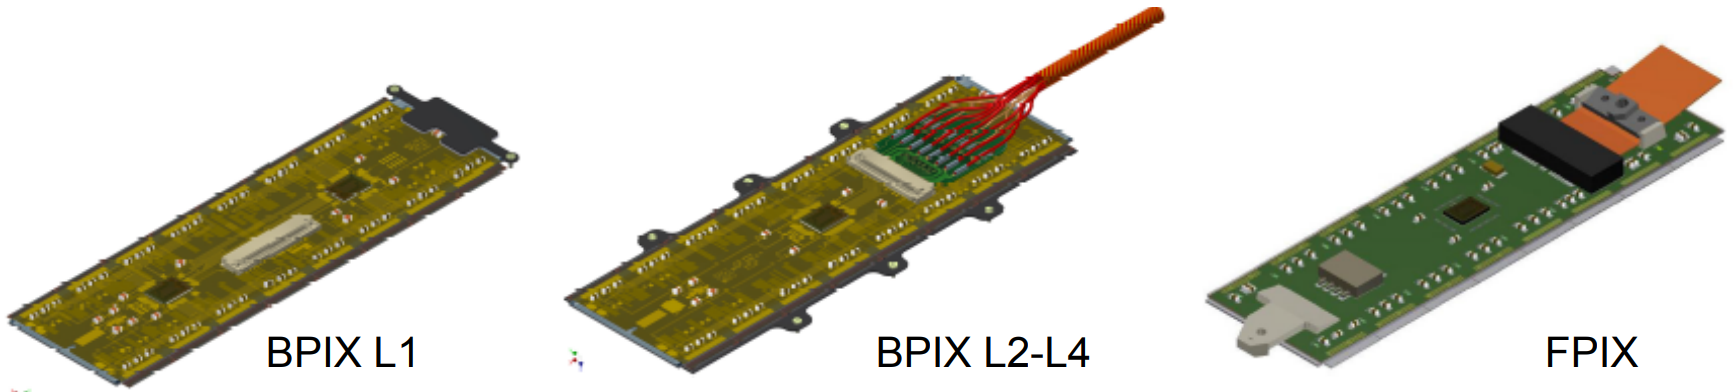
\includegraphics[scale=.2]{Chapter2/modules_drawing.png}
    \caption[Pixel detector modules]{ Drawings of the pixel detector modules for BPIX L1 (left), BPIX L2–4 (middle), and the FPIX detector (right)\cite{phase1_Pixel_Detector}.}
    \label{modules_drawing}
  \end{figure}
\end{center}

The track reconstruction process involves several steps. Firstly, zero-suppressed signals above specified thresholds in pixel channels are clustered into hits. These hit pixels are then combined to form clusters from neighboring pixels. The charge measured within each cluster corresponds to the charge deposited by a single charged particle. Next, the cluster positions and their uncertainties are estimated in a local orthogonal coordinate system $(u,v)$ in the plane of each sensor.\\

The pixel sensor used in this process consists of 100 $\times$ 150$\mu \text{m}^{2}$ pixels with the u-axis oriented parallel to the shorter pixel edge, this is shown en the figure \ref{module and hit}. To be considered a valid cluster, each one must have a minimum charge equivalent to 4000 electrons \cite{Track_Reco_2014,phase1_Pixel_Detector}.
For normally incident minimum-ionizing particles (MIPs) in a silicon sensor with a thickness of 285 $\mu \text{m}$, the most probable value of energy deposition corresponds to approximately 21000 electrons. However, this charge is often spread over more than one pixel due to Lorentz drift and diffusion of collected electrons, leading to charge clusters.\\

\begin{center}
  \begin{figure}[h]
    \centering
    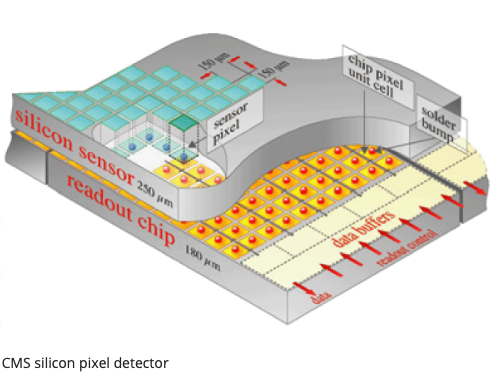
\includegraphics[scale=.3]{Chapter2/PixelSensor.png} 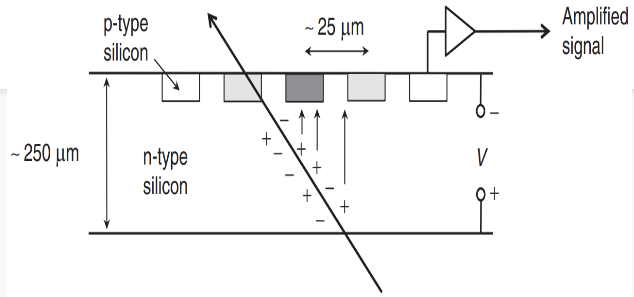
\includegraphics[scale=.3]{Chapter2/hit.png}
    \caption[PixelSensor]{ left: Pixel sensor diagram, right: hits detection in pixel sensor. }
    \label{module and hit}
  \end{figure}
\end{center}
\subsection{CMS Luminometers}
A total of seven systems are used for measuring luminosity at CMS. The Pixel Luminosity Telescope (PLT) and Fast Beam Conditions Monitor (BCM1F) are dedicated systems for luminosity measurement, while the hadronic forward calorimeter (HF) uses a dedicated readout on an existing system. Additionally, three other methods, the drift tube luminosity (DT), the pixel cluster counting method (PCC), and the vertex counting method (VTX), use data from existing parts of the CMS detector to perform a luminosity measurement using the main CMS DAQ system. The PCC measurement uses the data collected with the standard CMS trigger system with triggers requiring colliding bunches but not any specific event activity, known as "zero-bias" triggers. Finally, the RAMSES detectors are part of the LHC environmental protection and monitoring systems, but they can also be used to provide a luminosity measurement readout through Timber, the operational data and LHC logging service \cite{pas_18}.

The PLT is a dedicated system for measuring luminosity using silicon pixel sensors. There are a total of 48 sensors arranged into 16 “telescopes”,the rate of "triple coincidences," where a hit is observed in all three planes, is measured.

BCM1F comprises a total of 24 sensors mounted on the same carriage as the PLT, consisting of 10 silicon sensors, 10 polycrystalline diamond (pCVD) sensors, and 4 single-crystal diamond (sCVD) sensors.

The HF luminosity measurement uses a dedicated readout system installed in the HF calorimeter. Only two HF rings are used for luminosity measurement to ensure relatively uniform occupancy. Two algorithms are available: the first relies on the fraction of occupied towers (HFOC), and the second is based on the sum of the transverse energy ET (HFET).

Drift tube luminosity (DT), which uses the rate of muon track stubs in the muon barrel track finder and  RAMSES detectors, a CERN radiation and environmental monitoring system, although not designed as a luminometer, function quite well as a luminosity measurement, using the rate observed in the detectors (primarily photons within the energy range of 50 keV to 7 MeV). Another method is the pixel cluster counting (PCC), which will be described in more detail in chapter 3 \cite{pas_18}.